% Chapter Template

\chapter{MODI} % Main chapter title

\label{Chapter3} % Change X to a consecutive number; for referencing this chapter elsewhere, use \ref{ChapterX}

\lhead{Capítulo 3. \emph{MODI}} % Change X to a consecutive number; this is for the header on each page - perhaps a shortened title

%----------------------------------------------------------------------------------------
%	SECTION 1
%----------------------------------------------------------------------------------------

\begin{figure}[htbp]
	\centering
		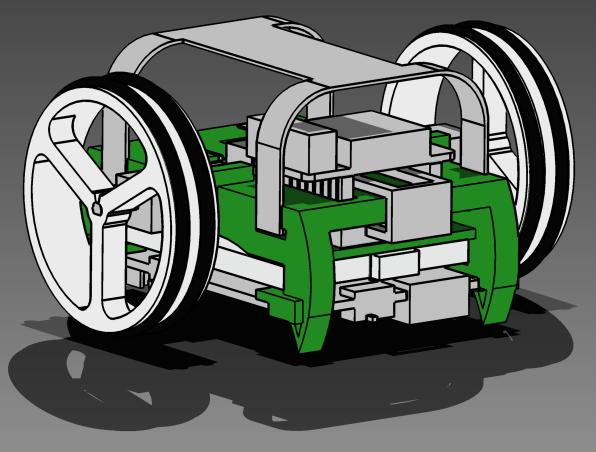
\includegraphics[width=0.8\textwidth]{./Figures/MODI/render.png}
		\rule{35em}{0.5pt}
	\caption[Setup]{robot MODI (sigla para Modular Intelligence)}
	\label{fig:MODI}
\end{figure}

\section{Setup}

Se desea realizar una investigación sobre el comportamiento colectivo de un grupo de robots, en el mundo real sin hacer uso de simuladores. Por esto  es necesario contar con un lugar físico donde poder activar los robot. Además para simplificar cada uno de los robots, estos no tienen sensores internos por lo que hay una cámara montada sobre el plano de movimiento de estos, para hacer Seguimiento Visual.
\begin{figure}[htbp]
	\centering
		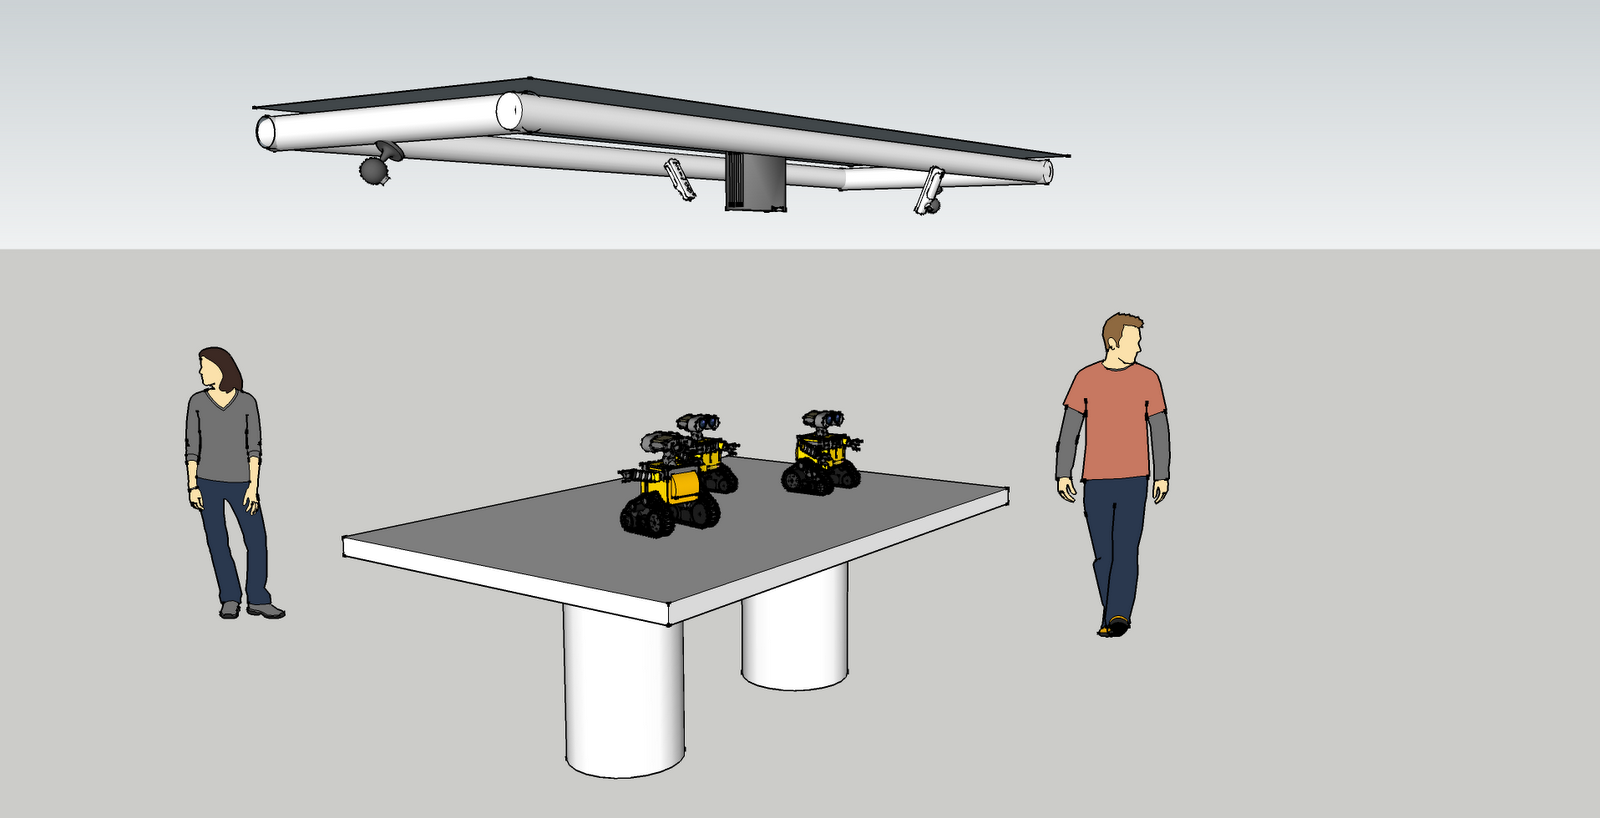
\includegraphics[width=0.8\textwidth]{./Figures/setup.png}
		\rule{35em}{0.5pt}
	\caption[Setup]{Setup a montarse para hacer estudios de grupos de robots.}
	\label{fig:setup}
\end{figure}

La función principal de MODI es ser una plataforma móvil de fácil acceso. Existe un repositorio en GitHub donde se tienen los códigos actualizados para controlar y construir robots MODI.  Para descargar códigos y piezas de construcción se debe ir a https://github.com/FabLabUCh/modi

\textbf{Las funciones principales que se desarrollaron}

\begin{itemize}
\item Carga Autónoma con celda solar.
\item Seguimiento de grupo.
\item Control individual del color de cada MODI.
\item Movimiento simple de cada robot de forma independiente.
\end{itemize}

%-----------------------------------
%	SECTION 2
%-----------------------------------

\section{Construcción}

%-----------------------------------
%	SUBSECTION 2
%-----------------------------------
\subsection{Fabricación Digital vs Análoga}
Cuando se quiere pasar una idea al mundo real es necesario un proceso de fabricación. Dependiendo de la cantidad de herramientas que se tenga es más o menos fácil la tarea. Desde el comienzo hasta hace un par de años, quienes se dedican a construir robots, debían construir de manera “artesanal” donde es imposible que las piezas queden todas iguales y el tiempo empleado era bastante. Hoy en día existe una gran alternativa que surge como un nuevo paradigma, la Fabricación Digital. Las impresoras 3D, que no son más que un extrusor montado en un sistema con ejes que le dan 3 grados de libertad, permiten desde un modelo hecho en un computador, obtener un objeto real en plástico. También existe otro tipo de máquinas que permite hacer diseños en 2D, estas son las cortadoras LASER. La primera versión de MODI fue construido usando planchas de madera MDF y acrílico, cortados en LASER.

\begin{figure}[htbp]
	\centering
		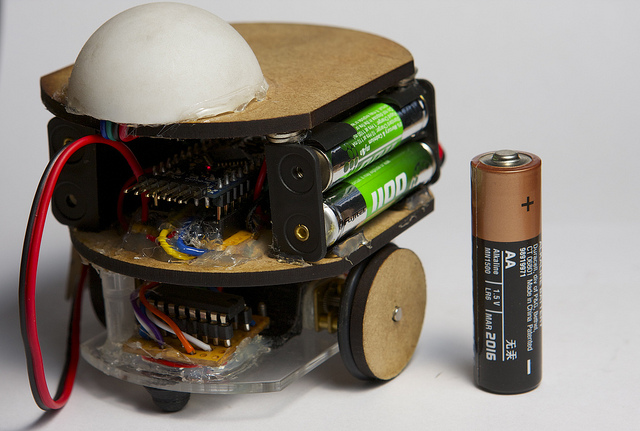
\includegraphics[width=0.8\textwidth]{./Pictures/MODIrev1.jpg}
		\rule{35em}{0.5pt}
	\caption[modi]{Primera versión robot MODI, tiene un Arduino mini pro, Xbee, usa pilas AAA y parte del chasis es de Madera MDF de 3[mm] cortado con LASER}
	\label{fig:modi1}
\end{figure}

\begin{figure}[htbp]
	\centering
		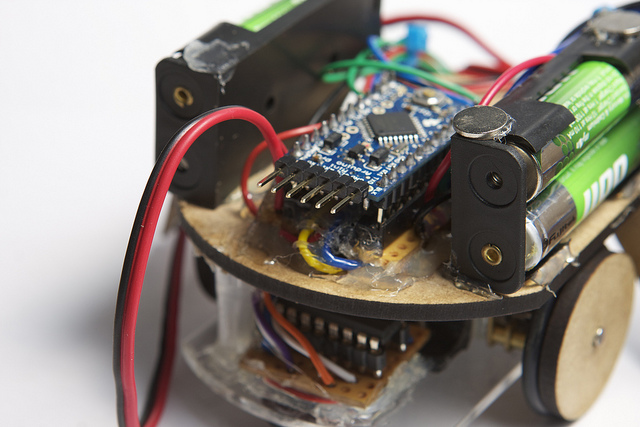
\includegraphics[width=0.8\textwidth]{./Pictures/2MODIrev1.jpg}
		\rule{35em}{0.5pt}
	\caption[modi2]{MODI, primera versión basada en gran parte en Fabricación Análoga.}
	\label{fig:modi2}
\end{figure}

Utilizando una impresora 3D Makerbot Replicator 1 se hizo esta primera versión con piezas plásticas.

\begin{figure}[htbp]
	\centering
		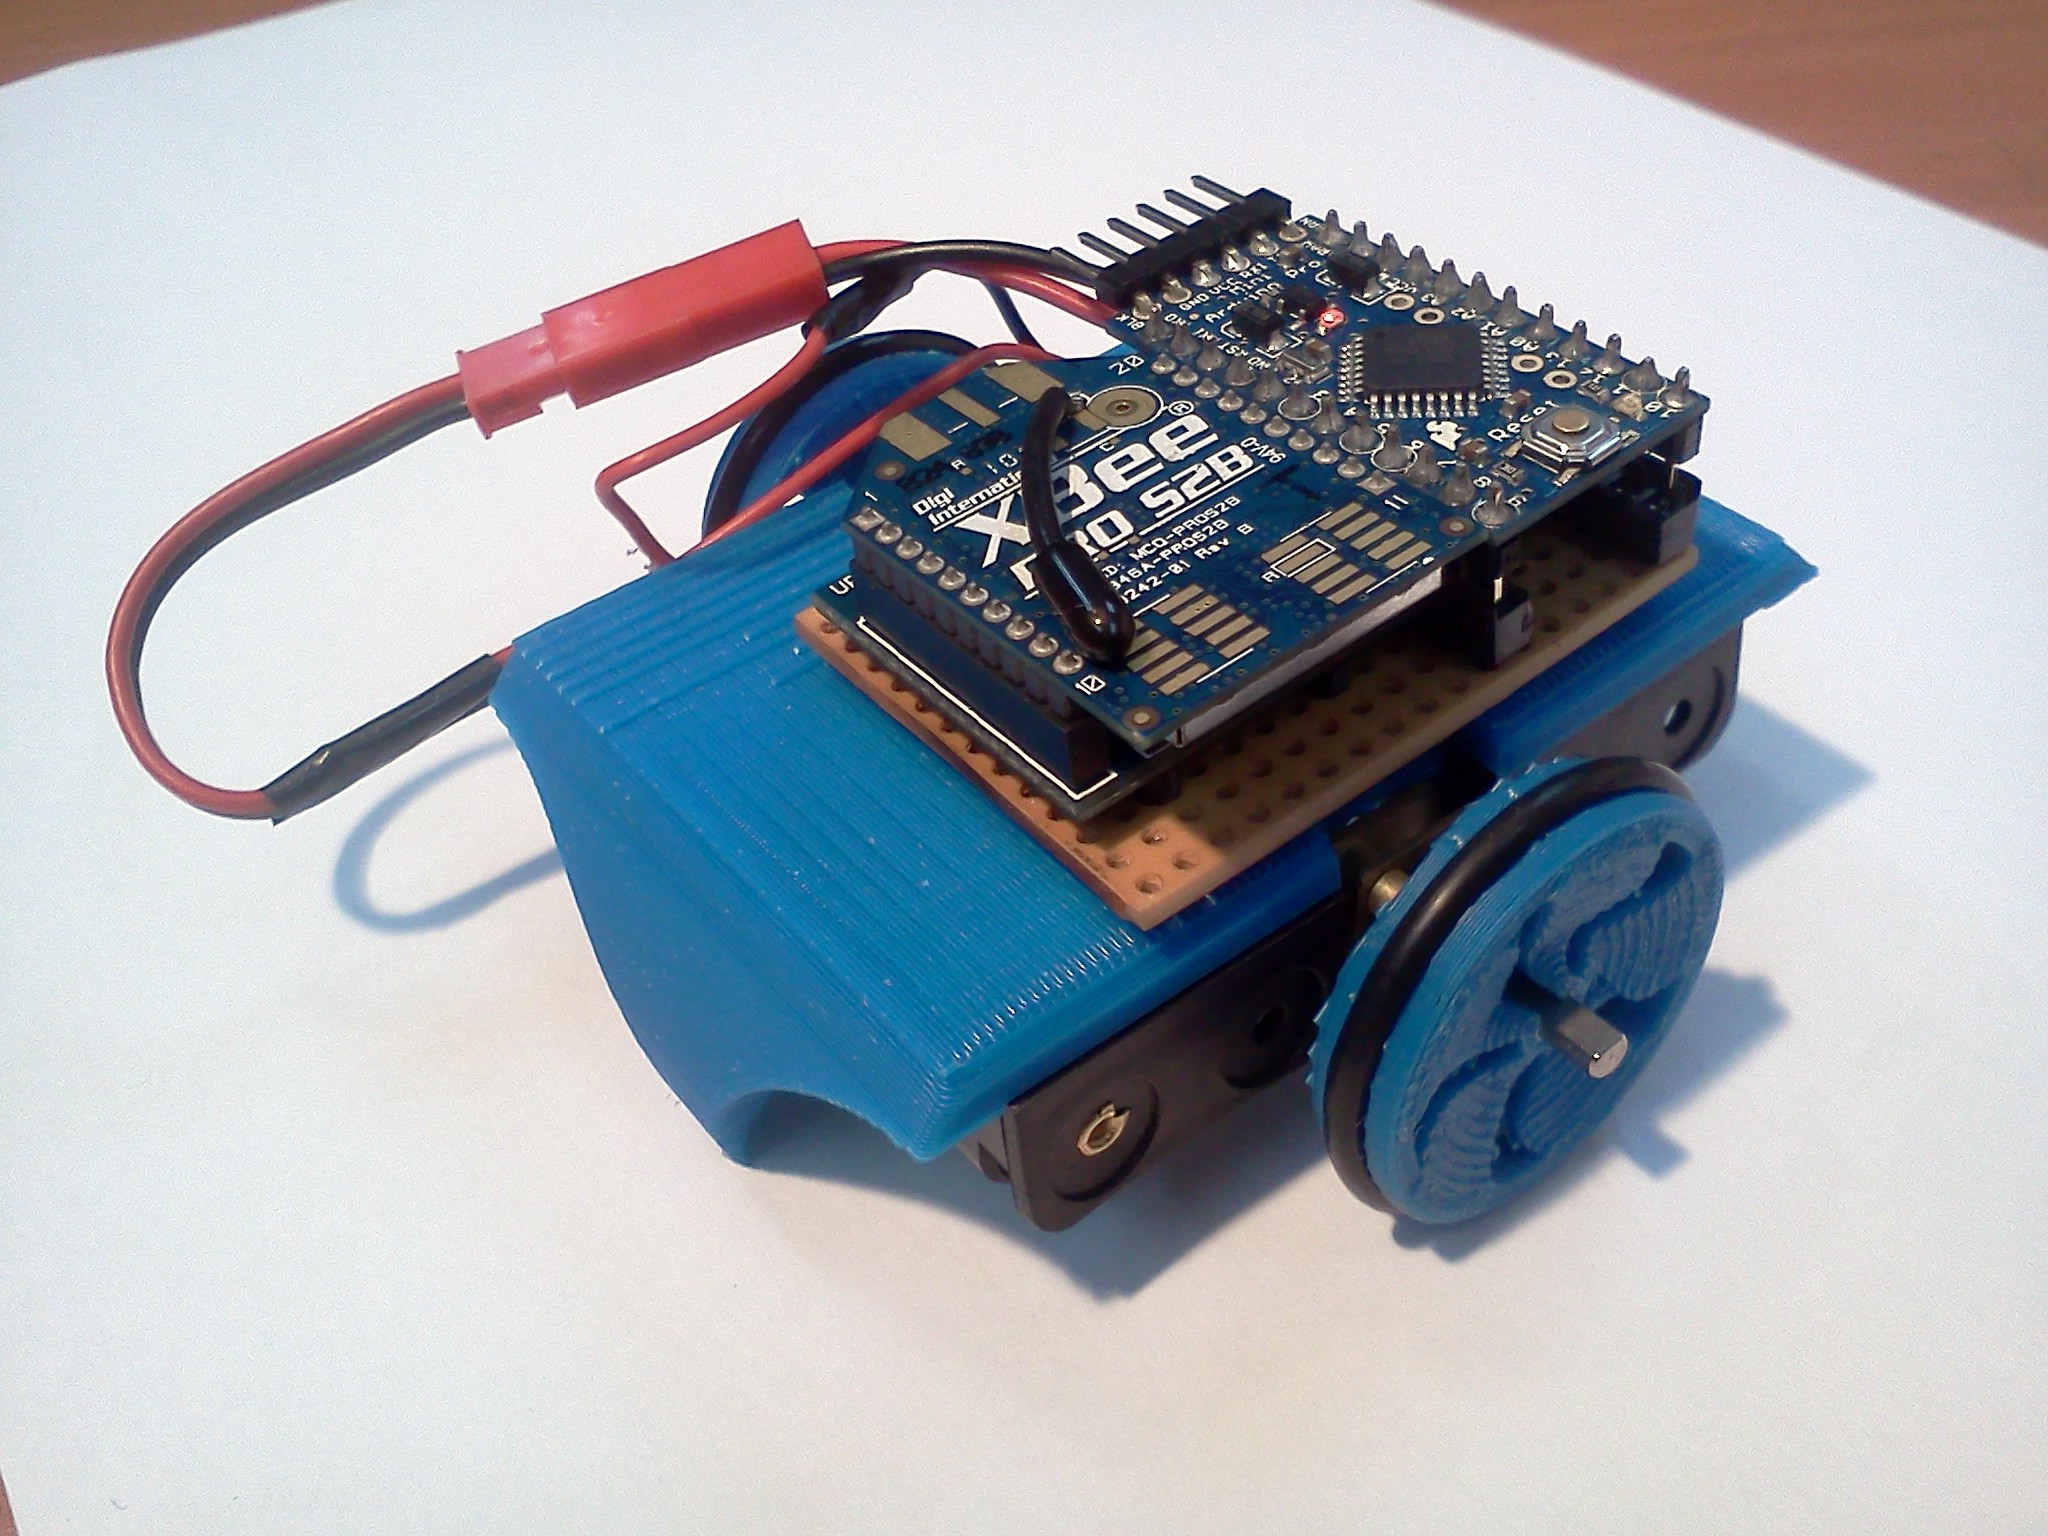
\includegraphics[width=0.8\textwidth]{./Pictures/MODIrev2.jpg}
		\rule{35em}{0.5pt}
	\caption[modirev1]{Primera versión de MODI usando técnica de \emph{ Fabricación Digital }con chasis de plástico construido con una MakerBot Replicator 1}
	\label{fig:modirev2}
\end{figure}

\begin{figure}[htbp]
	\centering
		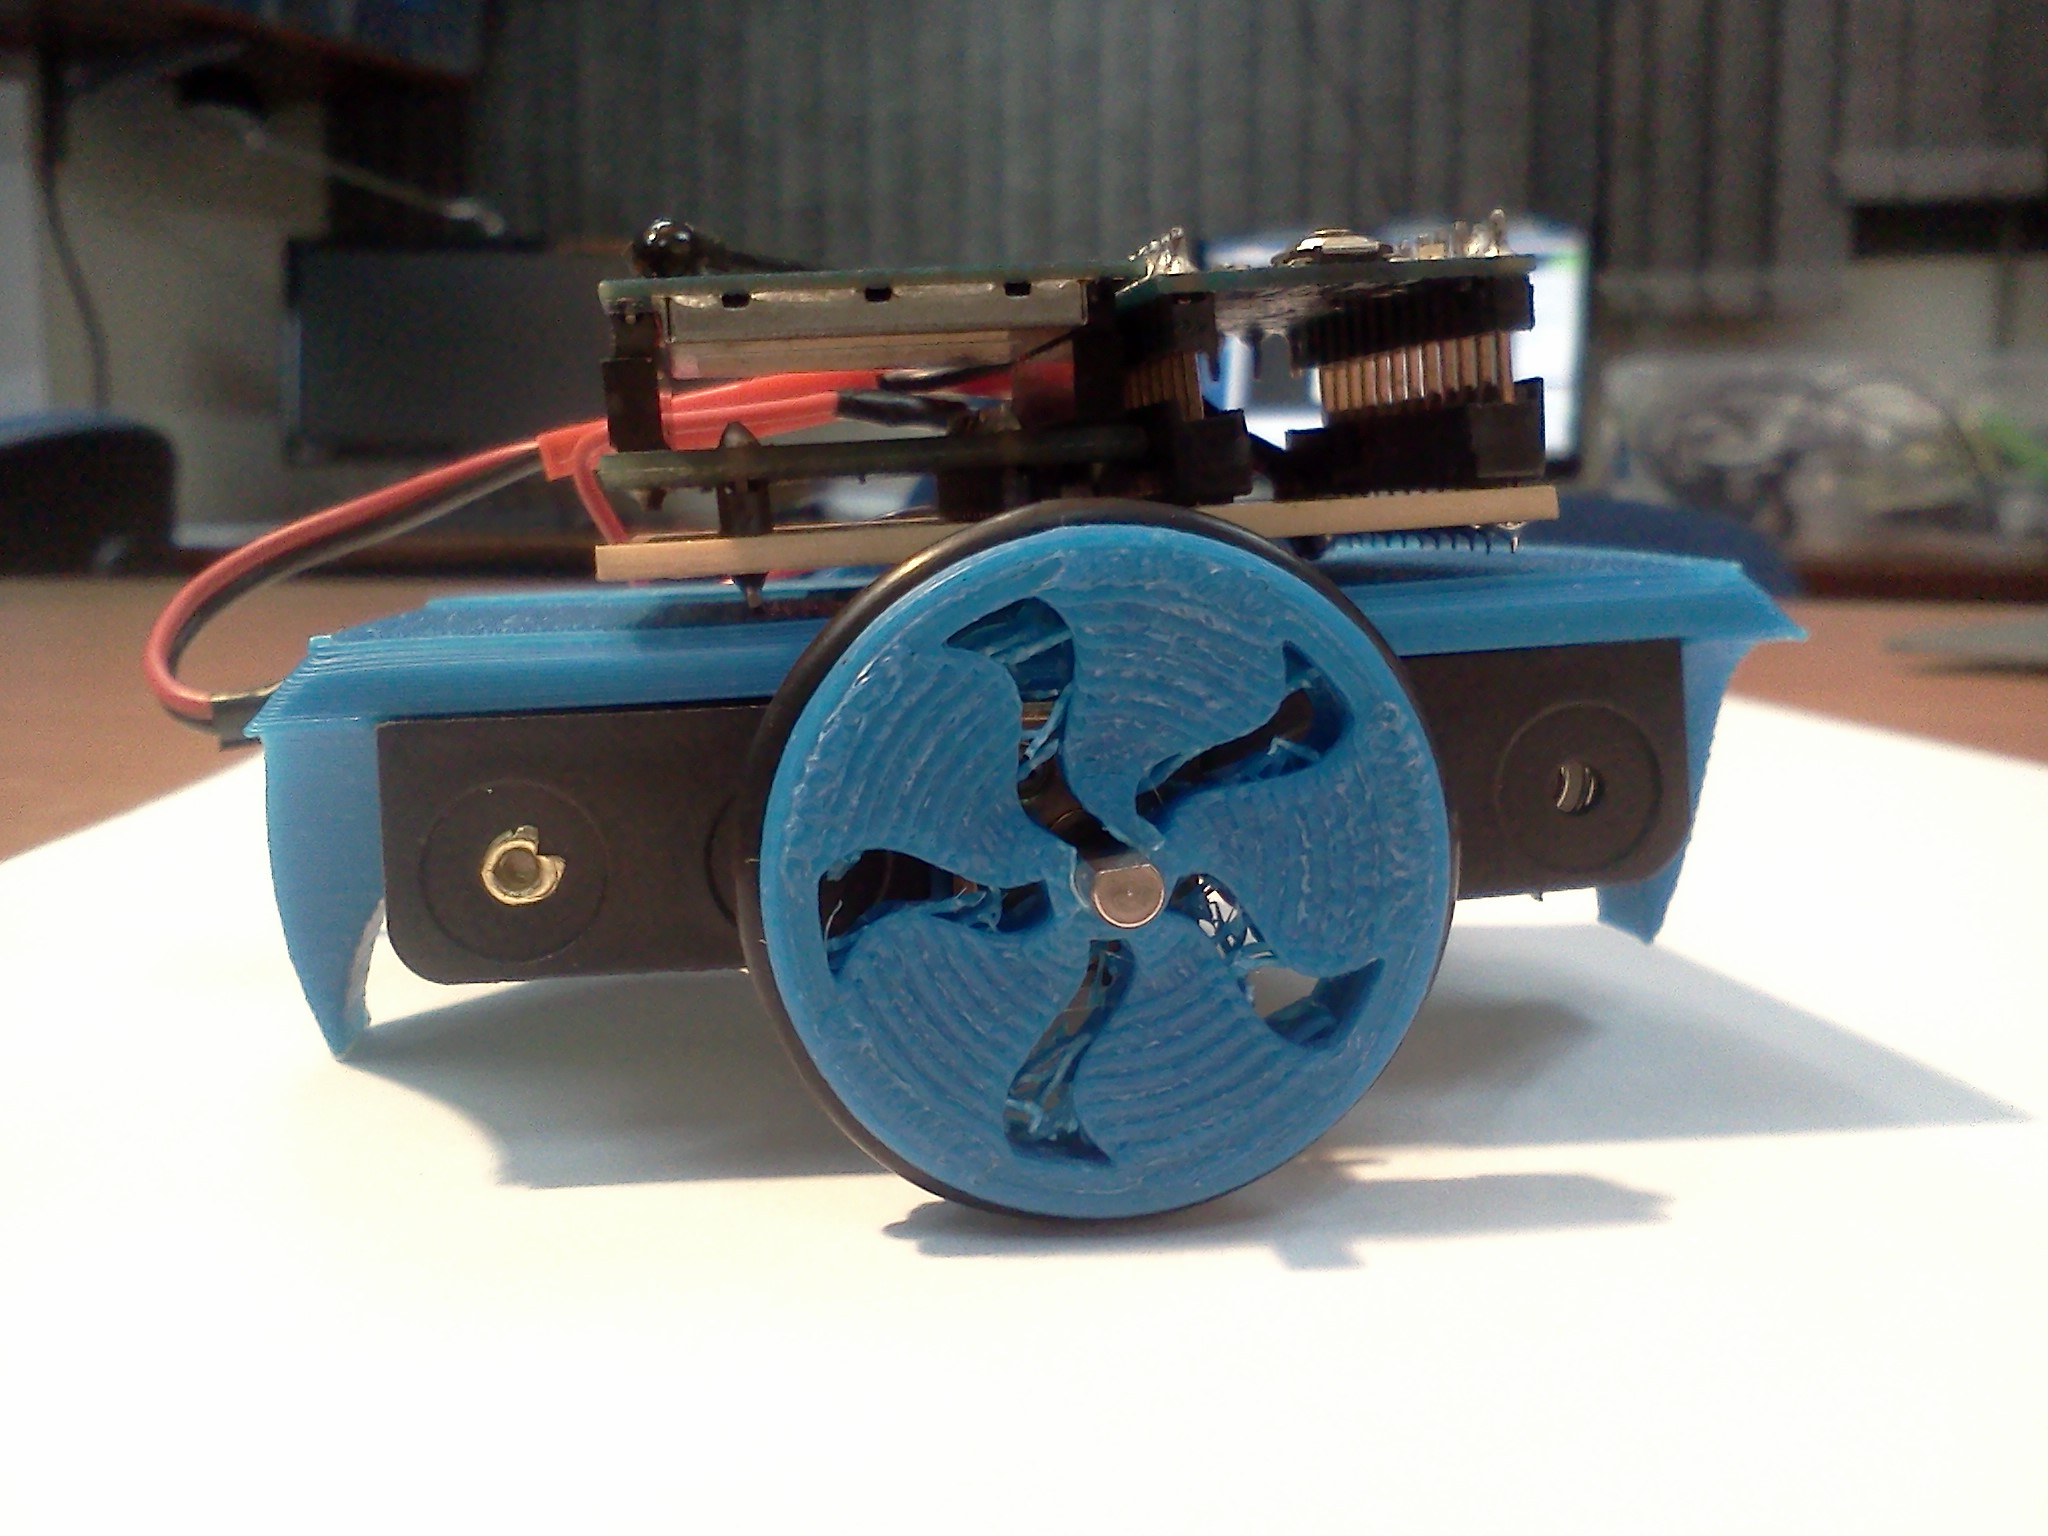
\includegraphics[width=0.8\textwidth]{./Pictures/2MODIrev2.jpg}
		\rule{35em}{0.5pt}
	\caption[modirev1]{Vista lateral.}
	\label{fig:2modirev2}
\end{figure}

\begin{figure}[htbp]
	\centering
		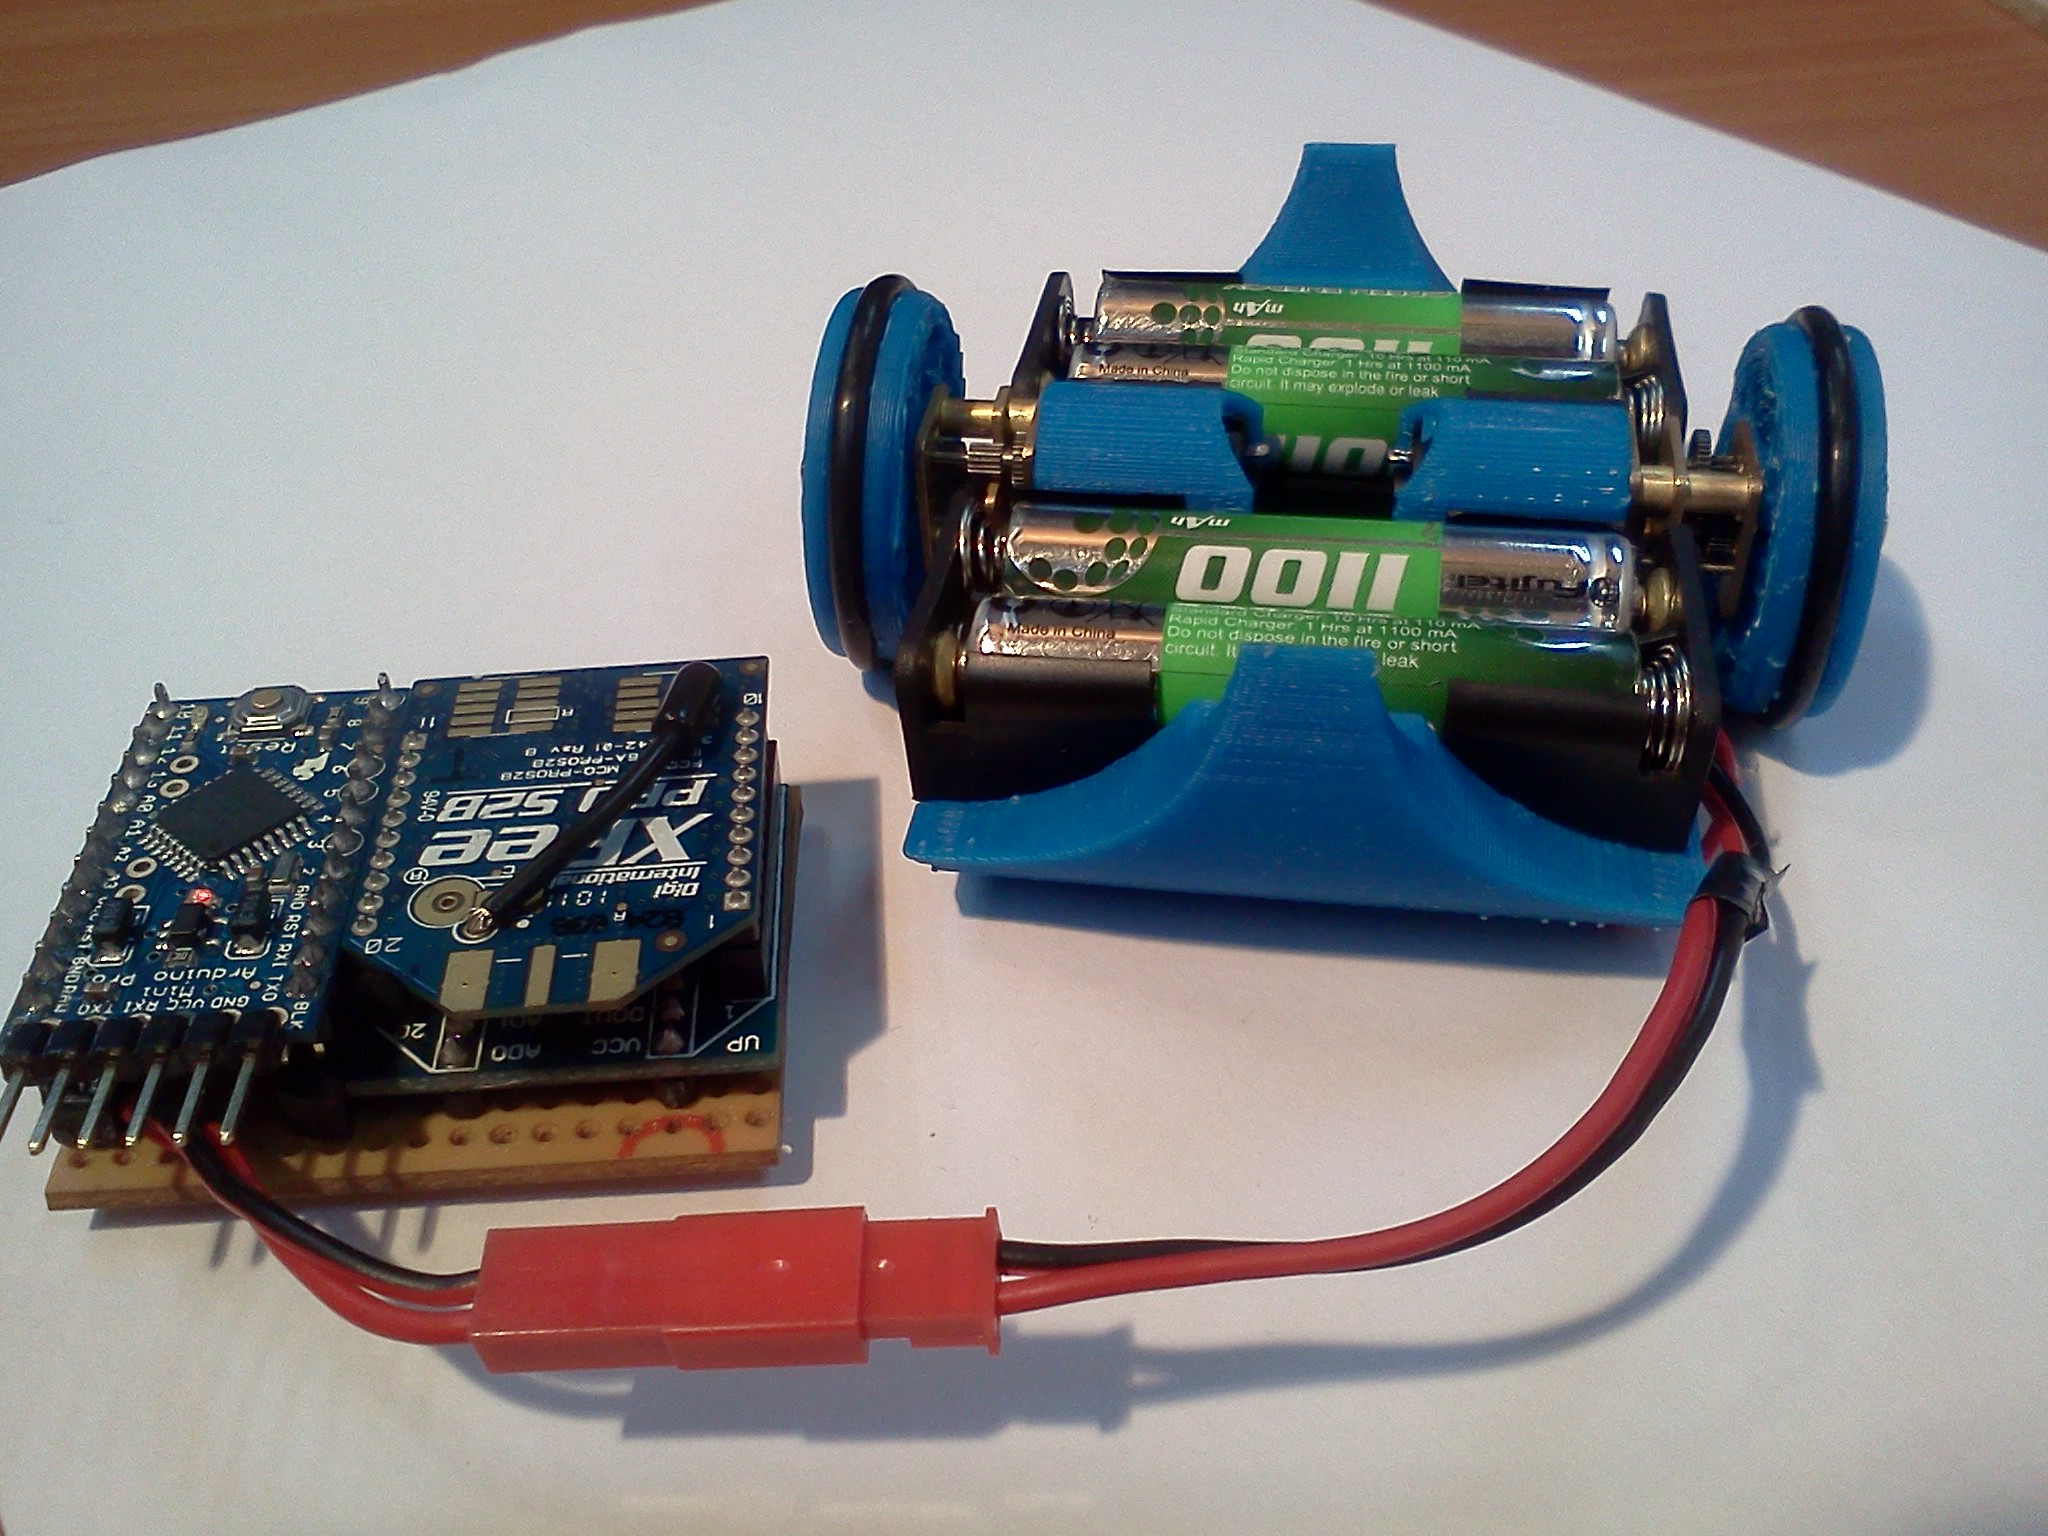
\includegraphics[width=0.8\textwidth]{./Pictures/3MODIrev2.jpg}
		\rule{35em}{0.5pt}
	\caption[modirev1]{Vista inferior.}
	\label{fig:3modirev2}
\end{figure}

Esta versión se dio de baja ya que presentaba el problema de involucrar demasiadas partes que debían ser hechas por una persona. El microcontrolador, junto con la radio inalámbrica se colocaron en una placa electrónica para prototipado, más adelante se puede ver que fueron reemplazados por una PCB llamada Arduino FIO. Otro factor clave para descartar esta versión es que utiliza 4 pilas AAA que necesitan ser removidas para poder ser recargadas, lo que impide que en futuras versión exista la posibilidad de una carga autónoma por parte de los Robots.

Aunque han bajado los precios de las maquinas para prototipado rápido, aún no están al alcance de todas las personas. Es por esto que existen los Fab labs (acrónimo del inglés Fabrication Laboratory), que según Wikipedia es, \textit{un espacio de producción de objetos físicos a escala personal o local que agrupa máquinas controladas por ordenadores. Su particularidad reside en su tamaño y en su fuerte vinculación con la sociedad.} Los Fab Labs están por todo el mundo, Figura \ref{fig:Fablabs}. MODI fue concebido como un proyecto del Fab Lab de la Universidad de Chile y por esto es posible reproducirlo en cualquier Fab Lab.

\begin{figure}[htbp]
	\centering
		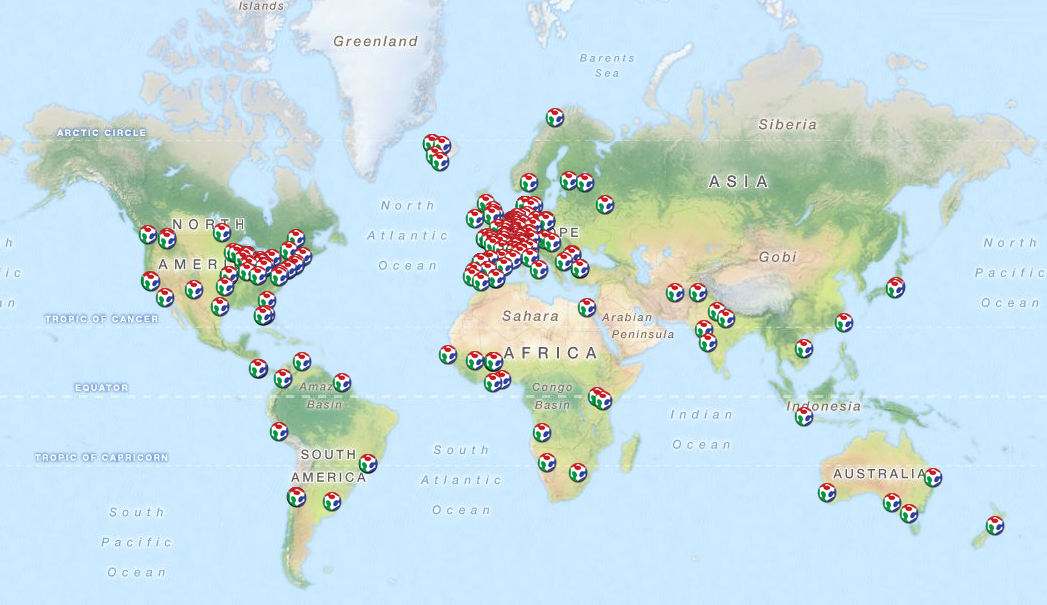
\includegraphics[width=0.8\textwidth]{./Figures/map.png}
		\rule{35em}{0.5pt}
	\caption[modirev1]{Mapa actual de lugares en el mundo que cuentan con un FabLab. En Chile a la fecha existen 3. Imagen obtenida desde http://fablabamersfoort.nl/fablabs/}
	\label{fig:Fablabs}
\end{figure}	

%-----------------------------------
%	SUBSECTION 3
%-----------------------------------
\subsection{Software CAD}

CAD viene de sus siglas del Inglés, Computer-aided design, y se refiere a un diseño asistido por herramientas computacionales. Profesionales como ingenieros, arquitectos y del área del diseño por lo general son los que hacen más uso de estas herramientas.

Según Wikipedia, \textit{”... se pueden dividir básicamente en programas de dibujo en dos dimensiones (2D) y modeladores en tres dimensiones (3D). Las herramientas de dibujo en 2D se basan en entidades geométricas vectoriales como puntos,líneas, arcos y polígonos, con las que se puede operar a través de una interfaz gráfica....”}

Durante el transcurso del proyecto se trabajó con varios softwares CAD. El primero fué SketchUp 8 de Google, que permite fácilmente hacer bocetos de lugares y cuenta con una importante biblioteca de modelos para incluir en el diseño. Rápidamente se pudo hacer un scketch utilizando modelos descargados de Internet , Figura~\ref{fig:setup}.

El diseño del chasis junto con las ruedas y demás partes plásticas, se hizo en un comienzo con SolidWorks 2012 y luego por ser más simple de usar, Inventor 2013 de Autodesk. Ambos softwares permiten generar modelos en 3D para luego exportar el diseño al formato STL que es estándar para prototipar en plástico.


\begin{figure}[htbp]
	\centering
		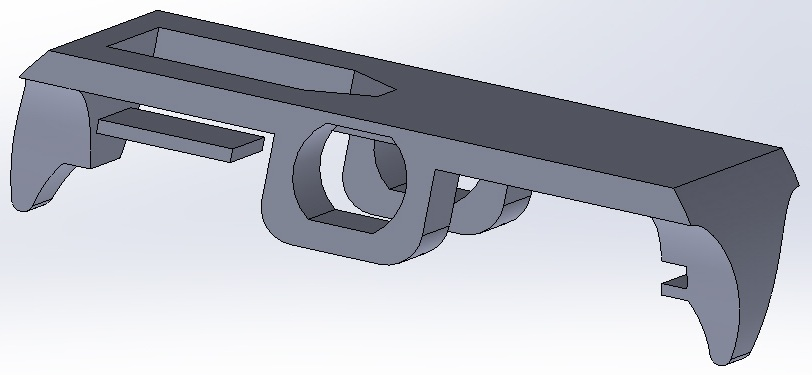
\includegraphics[width=0.8\textwidth]{./Figures/MODI/1MODI.jpg}
		\rule{35em}{0.5pt}
	\caption[ModiSolidWorks]{Primer Chasis de MODI, realizado con SolidWorks 2012. Esta versión sirve solo como prueba de concepto ya que no tiene espacio para las conexiones eléctricas necesarias}
	\label{fig:MODISolidWork}
\end{figure}	

Luego de varias iteraciones se lográ este modelo que tiene cinco piezas. 


\begin{figure}[htbp]
	\centering
		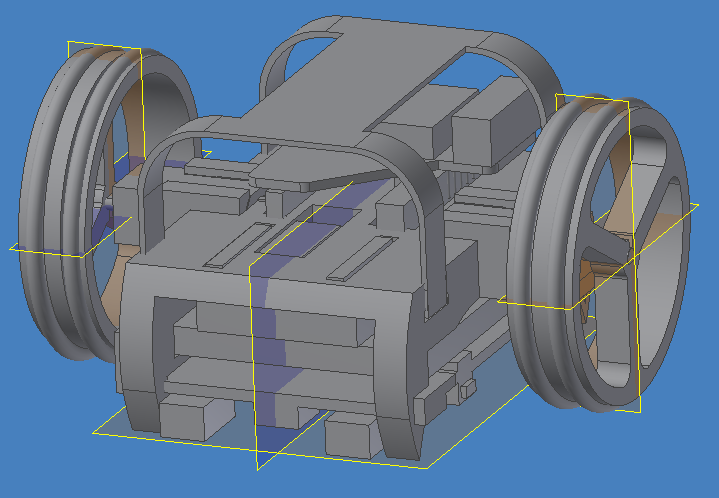
\includegraphics[width=0.8\textwidth]{./Figures/MODI/modi.png}
		\rule{35em}{0.5pt}
	\caption[Render]{Render de MODI realizado con Autodesk Inventor 2013.}
	\label{fig:MODIInventor}
\end{figure}

A continuación se describe cada una de ellas 

\begin{figure}[htbp]
	\centering
		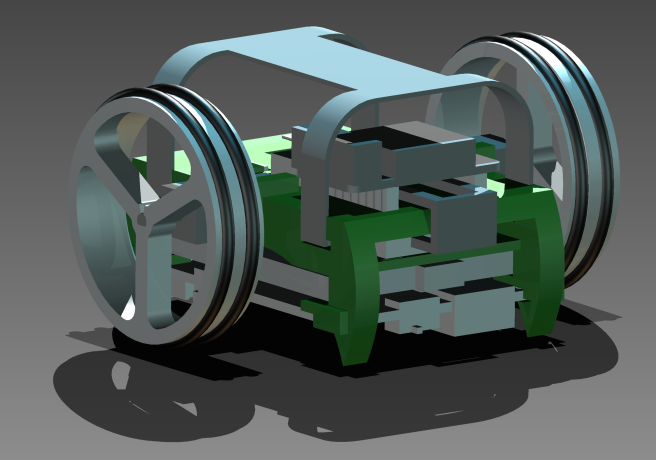
\includegraphics[width=0.8\textwidth]{./Figures/MODI/render2.png}
		\rule{35em}{0.5pt}
	\caption[Render]{Render de MODI realizado con Autodesk Inventor 2013.}
	\label{fig:render2}
\end{figure}	



